\documentclass[]{article}
\usepackage{lmodern}
\usepackage{setspace}
\setstretch{2}
\usepackage{amssymb,amsmath}
\usepackage{ifxetex,ifluatex}
\usepackage{fixltx2e} % provides \textsubscript
\ifnum 0\ifxetex 1\fi\ifluatex 1\fi=0 % if pdftex
  \usepackage[T1]{fontenc}
  \usepackage[utf8]{inputenc}
\else % if luatex or xelatex
  \ifxetex
    \usepackage{mathspec}
  \else
    \usepackage{fontspec}
  \fi
  \defaultfontfeatures{Ligatures=TeX,Scale=MatchLowercase}
\fi
% use upquote if available, for straight quotes in verbatim environments
\IfFileExists{upquote.sty}{\usepackage{upquote}}{}
% use microtype if available
\IfFileExists{microtype.sty}{%
\usepackage{microtype}
\UseMicrotypeSet[protrusion]{basicmath} % disable protrusion for tt fonts
}{}
\usepackage[margin=1in]{geometry}
\usepackage{hyperref}
\PassOptionsToPackage{usenames,dvipsnames}{color} % color is loaded by hyperref
\hypersetup{unicode=true,
            pdftitle={Component response rate variation underlies the stability of complex systems},
            pdfauthor={A. Bradley Duthie ( alexander.duthie@stir.ac.uk )},
            colorlinks=true,
            linkcolor=blue,
            citecolor=Blue,
            urlcolor=Blue,
            breaklinks=true}
\urlstyle{same}  % don't use monospace font for urls
\usepackage{graphicx,grffile}
\makeatletter
\def\maxwidth{\ifdim\Gin@nat@width>\linewidth\linewidth\else\Gin@nat@width\fi}
\def\maxheight{\ifdim\Gin@nat@height>\textheight\textheight\else\Gin@nat@height\fi}
\makeatother
% Scale images if necessary, so that they will not overflow the page
% margins by default, and it is still possible to overwrite the defaults
% using explicit options in \includegraphics[width, height, ...]{}
\setkeys{Gin}{width=\maxwidth,height=\maxheight,keepaspectratio}
\IfFileExists{parskip.sty}{%
\usepackage{parskip}
}{% else
\setlength{\parindent}{0pt}
\setlength{\parskip}{6pt plus 2pt minus 1pt}
}
\setlength{\emergencystretch}{3em}  % prevent overfull lines
\providecommand{\tightlist}{%
  \setlength{\itemsep}{0pt}\setlength{\parskip}{0pt}}
\setcounter{secnumdepth}{0}
% Redefines (sub)paragraphs to behave more like sections
\ifx\paragraph\undefined\else
\let\oldparagraph\paragraph
\renewcommand{\paragraph}[1]{\oldparagraph{#1}\mbox{}}
\fi
\ifx\subparagraph\undefined\else
\let\oldsubparagraph\subparagraph
\renewcommand{\subparagraph}[1]{\oldsubparagraph{#1}\mbox{}}
\fi

%%% Use protect on footnotes to avoid problems with footnotes in titles
\let\rmarkdownfootnote\footnote%
\def\footnote{\protect\rmarkdownfootnote}

%%% Change title format to be more compact
\usepackage{titling}

% Create subtitle command for use in maketitle
\newcommand{\subtitle}[1]{
  \posttitle{
    \begin{center}\large#1\end{center}
    }
}

\setlength{\droptitle}{-2em}

  \title{Component response rate variation underlies the stability of complex
systems}
    \pretitle{\vspace{\droptitle}\centering\huge}
  \posttitle{\par}
    \author{A. Bradley Duthie (
\href{mailto:alexander.duthie@stir.ac.uk}{\nolinkurl{alexander.duthie@stir.ac.uk}}
)}
    \preauthor{\centering\large\emph}
  \postauthor{\par}
      \predate{\centering\large\emph}
  \postdate{\par}
    \date{Biological and Environmental Sciences, University of Stirling, Stirling,
UK, FK9 4LA}

\usepackage{amsmath}
\usepackage{natbib}
\usepackage{lineno}
\usepackage[utf8]{inputenc}
\linenumbers
\bibliographystyle{amnatnat}

\begin{document}
\maketitle

\textbf{Key words:} Ecological networks, gene-regulatory networks,
neural networks, financial networks, system stability, random matrix
theory

\subsection{Abstract}\label{abstract}

The stability of a complex system generally decreases with increasing
system size and interconnectivity, a counterintuitive result of
widespread importance across the physical, life, and social sciences.
Despite recent interest in the relationship between system properties
and stability, the effect of variation in the response rate of
individual system components remains unconsidered. Here I vary the
component response rates (\(\boldsymbol{\gamma}\)) of randomly generated
complex systems. I show that when component response rates vary, the
potential for system stability is markedly increased. Variation in
\(\boldsymbol{\gamma}\) is especially important for stability in highly
complex systems, in which the probability of stability would otherwise
be negligible. At such extremes of simulated system complexity, the
largest stable complex systems would be unstable if not for
\(\boldsymbol{Var(\gamma)}\). My results therefore reveal a previously
unconsidered aspect of system stability that is likely to be pervasive
across all realistic complex systems.

\subsection{Introduction}\label{introduction}

In 1972, May\textsuperscript{\protect\hyperlink{ref-May1972}{1}} first
demonstrated that randomly assembled systems of sufficient complexity
are almost inevitably unstable given infinitesimally small
perturbations. Complexity in this case is defined by the size of the
system (i.e., the number of potentially interacting components; \(S\)),
its connectance (i.e., the probability that one component will interact
with another; \(C\)), and the variance of interaction strengths
(\(\sigma^{2}\))\textsuperscript{\protect\hyperlink{ref-Allesina2012}{2}}.
May's finding that the probability of local stability falls to near zero
given a sufficiently high threshold of \(\sigma\sqrt{SC}\) is broadly
relevant for understanding the dynamics and persistence of systems such
as
ecological\textsuperscript{\protect\hyperlink{ref-May1972}{1}--\protect\hyperlink{ref-Grilli2017}{5}},
neurological\textsuperscript{\protect\hyperlink{ref-Gray2008}{6},\protect\hyperlink{ref-Gray2009}{7}},
biochemical\textsuperscript{\protect\hyperlink{ref-Rosenfeld2009}{8},\protect\hyperlink{ref-MacArthur2010}{9}},
and
socio-economic\textsuperscript{\protect\hyperlink{ref-May2008}{10}--\protect\hyperlink{ref-Bardoscia2017}{13}}
networks. As such, identifying general principles that affect stability
in complex systems is of wide-ranging importance.

Randomly assembled complex systems can be represented as large square
matrices (\(\mathbf{M}\)) with \(S\) components (e.g., networks of
species\textsuperscript{\protect\hyperlink{ref-Allesina2012}{2}} or
banks\textsuperscript{\protect\hyperlink{ref-Haldane2011}{11}}). One
element of such a matrix, \(M_{ij}\), defines how component \(j\)
affects component \(i\) in the system at a point of
equilibrium\textsuperscript{\protect\hyperlink{ref-Allesina2012}{2}}.
Off-diagonal elements (\(i \neq j\)) therefore define interactions
between components, while diagonal elements (\(i = j\)) define component
self-regulation (e.g., carrying capacity in ecological communities).
Traditionally, off-diagonal elements are assigned non-zero values with a
probability \(C\), which are sampled from a distribution with variance
\(\sigma^{2}\); diagonal elements are set to
-1\textsuperscript{\protect\hyperlink{ref-May1972}{1},\protect\hyperlink{ref-Allesina2012}{2},\protect\hyperlink{ref-Allesina2015}{4}}.
Local system stability is assessed using eigenanalysis, with the system
being stable if the real parts of all eigenvalues (\(\lambda\)) of
\(\mathbf{M}\) are negative
(\(\max\left(\Re(\lambda)\right) < 0\))\textsuperscript{\protect\hyperlink{ref-May1972}{1},\protect\hyperlink{ref-Allesina2012}{2}}.
In a large system (high \(S\)), eigenvalues are distributed
uniformly\textsuperscript{\protect\hyperlink{ref-Tao2010}{14}} within a
circle centred at \(\Re = -1\) (the mean value of diagonal elements) and
\(\Im = 0\), with a radius of
\(\sigma\sqrt{SC}\)\textsuperscript{\protect\hyperlink{ref-May1972}{1},\protect\hyperlink{ref-Allesina2012}{2},\protect\hyperlink{ref-Allesina2015}{4}}
(Figs 1a and 2a). Local stability of randomly assembled systems
therefore becomes increasingly unlikely as \(S\), \(C\), and
\(\sigma^{2}\) increase.

May's\textsuperscript{\protect\hyperlink{ref-May1972}{1},\protect\hyperlink{ref-Allesina2012}{2}}
stability criterion \(\sigma\sqrt{SC} < 1\) assumes that the expected
response rates (\(\gamma\)) of individual components to perturbations of
the system are identical, but this is highly unlikely in any complex
system. In ecological communities, for example, the rate at which
population density changes following perturbation will depend on the
generation time of organisms, which might vary by orders of magnitude
among species. Species with short generation times will respond quickly
(high \(\gamma\)) to perturbations relative to species with long
generation times (low \(\gamma\)). Similarly, the speed at which
individual banks respond to perturbations in financial networks, or
individuals or institutions respond to perturbations in complex social
networks, is likely to vary. The effect of such variance on stability
has not been investigated in complex systems theory. Intuitively,
variation in \(\gamma\) might be expected to decrease system stability
by introducing a new source of variation into the system and thereby
increasing \(\sigma\). Here I show why, despite higher \(\sigma\),
realistic complex systems (such that \(S\) is high but finite) are
actually more likely to be stable if their individual component response
rates vary

\subsection{Results}\label{results}

\textbf{Component response rates of random complex systems}. Rows in
\(\mathbf{M}\) define how a given component \(i\) is affected by other
components of the system, meaning that the rate of component response
time can be modelled by multiplying all row elements by a real scalar
value
\(\gamma_{i}\)\textsuperscript{\protect\hyperlink{ref-Patel2018}{15}}.
The distribution of \(\gamma\) over \(S\) components thereby models the
distribution of component response rates. An instructive example
compares one \(\mathbf{M}\) where \(\gamma_{i} = 1\) for all \(i\) in
\(S\) to the same \(\mathbf{M}\) when half of \(\gamma_{i} = 1.95\) and
half of \(\gamma_{i} = 0.05\). This models one system in which
\(\gamma\) is invariant and one in which \(\gamma\) varies, but systems
are otherwise identical (note that mean \(\gamma_{i} = 1\) in both
cases). I assume \(S = 200\), \(C = 0.05\), and \(\sigma = 0.4\);
diagonal elements are set to \(-1\) and non-zero off-diagonal elements
are drawn randomly from \(\mathcal{N}(0, \sigma^{2})\). Rows are then
multiplied by \(\gamma_{i}\) to generate \(\mathbf{M}\). When
\(\gamma_{i} = 1\), eigenvalues of \(\mathbf{M}\) are distributed
uniformly within a circle centred at (\(-1, 0\)) with a radius of 1.265
(Fig. 1a). Hence, the real components of eigenvalues are highly unlikely
to all be negative when all \(\gamma_{i} = 1\). But when \(\gamma_{i}\)
values are separated into two groups, eigenvalues are no longer
uniformly distributed (Fig. 1b). Instead, two distinct clusters of
eigenvalues appear (red circles in Fig. 1b), one centred at
(\(-1.95, 0\)) and the other centred at (\(-0.05, 0\)). The former has a
large radius, but the real components have shifted to the left (in
comparison to when \(\gamma = 1\)), while the latter cluster has a
smaller radius, but real components have shifted to the right; all
\(\Re({\lambda}) < 0\). Overall, for 1 million randomly assembled
\(\mathbf{M}\), this division between slow and fast component response
rates results in more stable systems: 1 stable given \(\gamma = 1\)
versus 32 stable given \(\gamma = \{1.95, 0.5\}\).

Higher stability in systems with variation in \(\gamma\) can be observed
by sampling \(\gamma_{i}\) values from various distributions. I focus on
a uniform distribution where \(\gamma \sim \mathcal{U}(0, 2)\) (see
Supplementary Information for other distributions, which give similar
results). As with the case of \(\gamma = \{1.95, 0.5\}\) (Fig. 1b), mean
\(\gamma = 1\) when \(\gamma \sim \mathcal{U}(0, 2)\), allowing
comparison of \(\mathbf{M}\) before and after the addition of variation
in component response rate. Figure 2 shows a comparison of eigenvalue
distributions given \(S = 1000\), \(C = 0.05\), and \(\sigma = 0.4\). As
expected\textsuperscript{\protect\hyperlink{ref-Tao2010}{14}}, when
\(\gamma = 1\), eigenvalues are distributed uniformly in a circle
centred at (\(-1, 0\)) with a radius of \(\sigma\sqrt{SC} =\) 2.828.
Uniform variation in \(\gamma\) leads to a non-uniform distribution of
eigenvalues\textsuperscript{\protect\hyperlink{ref-Ahmadian2015}{16}--\protect\hyperlink{ref-Stone2017}{18}},
some of which are clustered locally near the centre of the distribution,
but others of which are spread outside the former radius of 2.828 (Fig
2b). The clustering and spreading of eigenvalues introduced by
\(Var(\gamma)\) can destabilise previously stable systems or stabilise
systems that are otherwise unstable. But where systems are otherwise too
complex to be stable given \(\gamma = 1\), the effect of \(Var(\gamma)\)
can often lead to stability above
May's\textsuperscript{\protect\hyperlink{ref-May1972}{1},\protect\hyperlink{ref-Allesina2012}{2}}
threshold \(\sigma\sqrt{SC} < 1\).

\textbf{Simulation of random \(\mathbf{M}\) across \(\mathbf{S}\)}. To
investigate the effect of \(Var(\gamma)\) on stability across systems of
varying complexity, I simulated random \(\mathbf{M}\) matrices at
\(\sigma = 0.4\) and \(C = 1\) across \(S = \{2, 3, ..., 49, 50\}\). One
million \(\mathbf{M}\) were simulated for each \(S\), and the stability
of \(\mathbf{M}\) was assessed given \(\gamma = 1\) versus
\(\gamma \sim \mathcal{U}(0, 2)\). For all \(S > 10\), I found that the
number of stable random systems was higher given \(Var(\gamma)\) than
when \(\gamma = 1\) (Fig. 3; see Supplementary Information for full
table of results), and that the difference between the probabilities of
observing a stable system increased with an increase in \(S\). In other
words, the potential for \(Var(\gamma)\) to affect stability increased
with system complexity and was most relevant for systems on the cusp of
being too complex to be realistically stable. For the highest values of
\(S\), nearly all systems that were stable given \(Var(\gamma)\) would
not have been stable given \(\gamma = 1\).

\textbf{Targeted manipulation of \(\mathbf{\gamma}\)}. To further
investigate the potential of \(Var(\gamma)\) to be stabilising, I used a
genetic algorithm. Genetic algorithms are heuristic tools that mimic
evolution by natural selection, and are useful when the space of
potential solutions (in this case, possible combinations of \(\gamma\)
values leading to stability in a complex system) is too large to search
exhaustively\textsuperscript{\protect\hyperlink{ref-Hamblin2013}{19}}.
Generations of selection on \(\gamma\) value combinations to minimise
\(\max\left(\Re(\lambda)\right)\) demonstrated the potential for
\(Var(\gamma)\) to increase system stability. Across
\(S = \{2, 3, ..., 39, 40\}\), sets of \(\gamma\) values were found that
resulted in stable systems with probabilities that were up to four
orders of magnitude higher than when \(\gamma = 1\) (Fig. 4), meaning
that stability could often be achieved by manipulating \(S\) \(\gamma\)
values rather than \(S \times S\) \(\mathbf{M}\) elements (i.e., by
manipulating component response rates rather than interactions between
components).

\textbf{System feasibility given \(\mathbf{Var(\gamma)}\)} For complex
systems in which individual system components represent the density of
some tangible quantity, it is relevant to consider the feasibility of
the system. Feasibilility assumes that values of all components are
positive at
equilibrium\textsuperscript{\protect\hyperlink{ref-Grilli2017}{5},\protect\hyperlink{ref-Dougoud2018}{20},\protect\hyperlink{ref-Song2018}{21}}.
This is of particular interest for ecological communities because
population density (\(N\)) cannot take negative values, meaning that
ecological systems need to be feasible for stability to be biologically
realistic\textsuperscript{\protect\hyperlink{ref-Dougoud2018}{20}}.
While my results are intended to be general to all complex systems, and
not restricted to species networks, I have also performed a feasibility
analysis on all matrices \(\mathbf{M}\) tested for stability, and
additionally for specific types of ecological
communities\textsuperscript{\protect\hyperlink{ref-Allesina2012}{2}}
(e.g., competitive, mutualist, predator-prey; see Supplementary
Information). I emphasise that \(\gamma\) is not interpreted as
population density in this analysis, but instead as a fundamental
property of species life history such as expected generation time.
Feasibility was unaffected by \(Var(\gamma)\) and instead occurred with
a fixed probability of \(1/2^{S}\), consistent with a recent proof by
Serván et al.\textsuperscript{\protect\hyperlink{ref-Servan2018}{22}}
(see Supplementary Information). Hence, for pure interacting species
networks, variation in component response rate (i.e., species generation
time) does not affect stability at biologically realistic species
densities.

\subsection{Discussion}\label{discussion}

I have shown that the stability of complex systems might often be
contigent upon variation in the response rates of their individual
components, meaning that factors such as rate of trait evolution (in
biological networks), transaction speed (in economic networks), or
communication speed (in social networks) need to be considered when
investigating the stability of complex systems. Variation in component
response rate is more likely to be critical for stability in systems
that are especially complex, and it can ultimately increase the
probability that system stability is observed above that predicted by
May's\textsuperscript{\protect\hyperlink{ref-May1972}{1}} classically
derived \(\sigma \sqrt{SC}\) criterion. The logic outlined here is
general, and potentially applies to any complex system in which
individual system components can vary in their reaction rates to system
perturbation.

It is important to recognise that variation in component response rate
is not stabilising per se; that is, adding variation in component
response rates to a particular system does not increase the probability
that the system will be stable. Rather, highly complex systems that are
observed to be stable are more likely to have varying component response
rates, and for this variation to be critical to their stability (Fig.
3). This is caused by the shift to a non-uniform distribution of
eigenvalues that occurs by introducing \(Var(\gamma)\) (Fig. 1b, 2b),
which can sometimes cause all of the real components of the eigenvalues
of the system matrix to become negative, but might also increase the
real components of eigenvalues.

My focus is distinct from Gibbs et
al.\textsuperscript{\protect\hyperlink{ref-Gibbs2017}{17}}, who applied
the same mathematical framework to investigate how a diagonal matrix
\(\mathbf{X}\) (equivalent to \(\gamma\) in my model) affects the
stability of a community matrix \(\mathbf{M}\) given an interaction
matrix \(\mathbf{A}\) within a generalised Lotka-Volterra model, where
\(\mathbf{M} = \mathbf{XA}\). Gibbs et
al.\textsuperscript{\protect\hyperlink{ref-Gibbs2017}{17}} analytically
demonstrated that the effect of \(\mathbf{X}\) on system stability
decreases exponentially as system size becomes arbitrarily large
(\(S \to \infty\)) for a given magnitude of complexity
\(\sigma\sqrt{SC}\). My numerical results do not contradict this
prediction because I did not scale \(\sigma = 1 / \sqrt{S}\), but
instead fixed \(\sigma\) and increased \(S\) to thereby increase total
system complexity (see Supplemental Information for results simulated
across \(\sigma\) and \(C\)). Overall, I show that component response
rate variation increases the upper bound of complexity at which
stability can be realistically observed, meaning that highly complex
systems are more likely than not to vary in their component response
rates, and for this variation to be critical for system stability.

The potential importance of component response rate variation was most
evident from the results of simulations in which the genetic algorithm
was used in attempt to maximise the probability of system stability. The
probability that some combination of component response rates could be
found to stabilise the system was shown to be up to four orders of
magnitude higher than the background probabilities of stability in the
absence of any component response rate variation. Instead of
manipulating the \(S \times S\) interactions between system components,
it might therefore be possible to manipulate only the \(S\) response
rates of individual system components to achieve stability. Hence,
managing the response rates of system components in a targeted way could
potentially facilitate the stabilisation of complex systems through a
reduction in dimensionality.

Interestingly, while complex systems were more likely to be stable given
variation in component response rate, they were not more likely to be
feasible, meaning that stability was not increased when component values
were also restricted to being positive at equilibrium. Feasibility is
important to consider, particularly for the study of ecological networks
of
species\textsuperscript{\protect\hyperlink{ref-Grilli2017}{5},\protect\hyperlink{ref-Stone2017}{18},\protect\hyperlink{ref-Dougoud2018}{20},\protect\hyperlink{ref-Servan2018}{22}}
because population densities cannot realistically be negative. My
results therefore suggest that variation in the rate of population
responses to perturbation (e.g., due to differences in generation time
among species) is unlikely to be critical to the stability of purely
multi-species interaction networks (see also Supplementary Information).
Nevertheless, ecological interactions do not exist in isolation in
empirical
systems\textsuperscript{\protect\hyperlink{ref-Patel2018}{15}}, but
instead interact with evolutionary, abiotic, or social-economic systems.
The relevance of component response rate for complex system stability
should therefore not be ignored in the broader context of ecological
communities.

A general mathematical framework encompassing shifts in eigenvalue
distributions caused by a vector \(\gamma\) has been
investigated\textsuperscript{\protect\hyperlink{ref-Ahmadian2015}{16}}
and recently applied to questions concerning species density and
feasibility\textsuperscript{\protect\hyperlink{ref-Gibbs2017}{17},\protect\hyperlink{ref-Stone2017}{18}},
but \(\gamma\) has not been interpreted as rates of response of
individual system components to perturbation. My model focuses on
component response rates for systems of a finite size, in which
complexity is high but not yet high enough to make the probability of
stability unrealistically low for actual empirical systems. For this
upper range of system size, randomly assembled complex systems are more
likely to be stable if their component response rates vary (e.g.,
\(10 < S < 30\) for parameter values in Fig. 3). Overall, I suggest that
variation in component response rate might therefore be critical for
maintaining stability in many highly complex empirical systems. These
results are broadly applicable for understanding the stability of
complex networks across the physical, life, and social sciences.

\subsection{Methods}\label{methods}

\textbf{Component response rate variation (\(\mathbf{\gamma}\))}. In a
synthesis of eco-evolutionary feedbacks on community stability, Patel et
al. model a system that includes a vector of potentially changing
species densities (\(\mathbf{N}\)) and a vector of potentially evolving
traits
(\(\mathbf{x}\))\textsuperscript{\protect\hyperlink{ref-Patel2018}{15}}.
For any species \(i\) or trait \(j\), change in species density
(\(N_{i}\)) or trait value (\(x_{j}\)) with time (\(t\)) is a function
of the vectors \(\mathbf{N}\) and \(\mathbf{x}\),

\[\frac{dN_{i}}{dt} = N_{i}f_{i}(\mathbf{N}, \mathbf{x}),\]

\[\frac{dx_{j}}{dt} = \epsilon g_{j}(\mathbf{N}, \mathbf{x}).\]

In the above, \(f_{i}\) and \(g_{j}\) are functions that define the
effects of all species densities and trait values on the density of a
species \(i\) and the value of trait \(j\), respectively. Patel et al.
were interested in stability when the evolution of traits was relatively
slow or fast in comparison with the change in species
densities\textsuperscript{\protect\hyperlink{ref-Patel2018}{15}}, and
this is modulated in the above by the scalar \(\epsilon\). The value of
\(\epsilon\) thereby determines the timescale separation between ecology
and evolution, with high \(\epsilon\) modelling relatively fast
evolution and low \(\epsilon\) modelling relative slow
evolution\textsuperscript{\protect\hyperlink{ref-Patel2018}{15}}.

I use the same principle that Patel et al. use to modulate the relative
rate of evolution to modulate rates of component responses for \(S\)
components. Following
May\textsuperscript{\protect\hyperlink{ref-May1972}{1},\protect\hyperlink{ref-May1973}{23}},
the value of a component \(i\) at time \(t\) (\(v_{i}(t)\)) is affected
by the value of \(j\) (\(v_{j}(t)\)) and \(j\)'s marginal effect on
\(i\) (\(a_{ij}\)), and by \(i\)'s response rate (\(\gamma_{i}\)),

\[\frac{dv_{i}(t)}{dt} = \gamma_{i} \sum_{j=1}^{S}a_{ij}v_{j}(t).\]

In matrix notation\textsuperscript{\protect\hyperlink{ref-May1973}{23}},

\[\frac{d\mathbf{v}(t)}{dt} = \mathbf{\gamma} \mathbf{A}\mathbf{v}(t).\]

In the above, \(\mathbf{\gamma}\) is a diagonal matrix in which elements
correspond to individual component response rates. Therefore,
\(\mathbf{M} = \mathbf{\gamma} \mathbf{A}\) defines the values of system
components and can be analysed using the techniques of
May\textsuperscript{\protect\hyperlink{ref-May1972}{1},\protect\hyperlink{ref-Ahmadian2015}{16},\protect\hyperlink{ref-May1973}{23}}.
In these analyses, row means of \(\mathbf{A}\) are expected to be
identical, but variation around this expectation will naturally arise
due to random sampling of \(\mathbf{A}\) off-diagonal elements and
finite \(S\). In simulations, the total variation in \(\mathbf{M}\) row
means that is attributable to \(\mathbf{A}\) is small relative to that
attributable to \(\mathbf{\gamma}\), especially at high \(S\). Variation
in \(\mathbf{\gamma}\) specifically isolates the effects of differing
component response rates, hence causing differences in expected
\(\mathbf{M}\) row means.

\textbf{Genetic algorithm}. Ideally, to investigate the potential of
\(Var(\gamma)\) for increasing the proportion of stable complex systems,
the search space of all possible \(\gamma\) vectors would be evaluated
for each unique \(\mathbf{M = \gamma A}\). This is technically
impossible because \(\gamma_{i}\) can take any real value between 0-2,
but even rounding \(\gamma_{i}\) to reasonable values would result in a
search space too large to practically explore. Under these conditions,
genetic algorithms are highly useful tools for finding practical
solutions by mimicking the process of biological
evolution\textsuperscript{\protect\hyperlink{ref-Hamblin2013}{19}}. In
this case, the practical solution is finding vectors of
\(\mathbf{\gamma}\) that decrease the most positive real eigenvalue of
\(\mathbf{M}\). The genetic algorithm used achieves this by initialising
a large population of 1000 different potential \(\mathbf{\gamma}\)
vectors and allowing this population to evolve through a process of
mutation, crossover (swaping \(\gamma_{i}\) values between vectors),
selection, and reproduction until either a \(\mathbf{\gamma}\) vector is
found where all \(\Re(\lambda) < 0\) or some ``giving up'' critiera is
met.

For each \(S = \{2, 3, ..., 39, 40\}\), the genetic algorithm was run
for 100000 random \(\mathbf{M}\) (\(\sigma = 0.4\), \(C = 1\)). The
genetic algorithm was initialised with a population of 1000 different
\(\mathbf{\gamma}\) vectors with elements sampled i.i.d from
\(\gamma_{i} \sim \mathcal{U}(0, 2)\). Eigenanalysis was performed on
the \(\mathbf{M}\) resulting from each \(\mathbf{\gamma}\) vector, and
the 20 \(\mathbf{\gamma}\) vectors resulting in \(\mathbf{M}\) with the
lowest \(\max\left(\Re(\lambda)\right)\) each produced 50 clonal
offspring with subsequent random mutation and crossover between the
resulting new generation of 1000 \(\mathbf{\gamma}\) vectors. Mutation
of each \(\gamma_{i}\) in a \(\mathbf{\gamma}\) vector occurred with a
probability of 0.2, resulting in a mutation effect of size
\(\mathcal{N}(0, 0.02)\) being added to generate the newly mutated
\(\gamma_{i}\) (any \(\gamma_{i}\) values that mutated below zero were
multiplied by \(-1\), and any values that mutated above 2 were set to
2). Crossover occurred between two sets of 100 \(\mathbf{\gamma}\)
vectors paired in each generation; vectors were randomly sampled with
replacement among but not within sets. Vector pairs selected for
crossover swapped all elements between and including two \(\gamma_{i}\)
randomly selected with replacement (this allowed for reversal of vector
element positions during crossover; e.g.,
\(\{\gamma_{4}, \gamma_{5}, \gamma_{6}, \gamma_{7}\} \to \{\gamma_{7}, \gamma_{6}, \gamma_{5}, \gamma_{4}\}\)
). The genetic algorithm terminated if a stable \(\mathbf{M}\) was
found, 20 generations occurred, or if the mean \(\mathbf{\gamma}\)
fitness increase between generations was less than 0.01 (where fitness
was defined as \(W_{\gamma} = -\max\left(\Re(\lambda)\right)\) for
\(\mathbf{M}\)).

\textbf{System feasibility}. Dougoud et
al.\textsuperscript{\protect\hyperlink{ref-Dougoud2018}{20}} identify
the following feasibility criteria for ecological systems characterised
by \(S\) interacting species with varying densities in a generalised
Lotka-Volterra model,

\[\mathbf{n^{*}} = -\left(\theta \mathbf{I} + (CS)^{-\delta}\mathbf{J} \right)^{-1}\mathbf{r}.\]

In the above, \(\mathbf{n^{*}}\) is the vector of species densities at
equilibrium. Feasibility is satisfied if all elements in
\(\mathbf{n^{*}}\) are positive. The matrix \(\mathbf{I}\) is the
identity matrix, and the value \(\theta\) is the strength of
intraspecific competition (diagonal elements). Diagonal values are set
to \(-1\), so \(\theta = -1\). The variable \(\delta\) is a
normalisation parameter that modulates the strength of interactions
(\(\sigma\)) for \(\mathbf{J}\). Implicitly, here \(\delta = 0\)
underlying strong interactions. Hence, \((CS)^{-\delta} = 1\), so in the
above, a diagonal matrix of -1s (\(\theta \mathbf{I}\)) is added to
\(\mathbf{J}\), which has a diagonal of all zeros and an off-diagonal
affecting species interactions (i.e., the expression \((CS)^{-\delta}\)
relates to May's\textsuperscript{\protect\hyperlink{ref-May1972}{1}}
stability
criterion\textsuperscript{\protect\hyperlink{ref-Dougoud2018}{20}} by
\(\frac{\sigma}{(CS)^{-\delta}}\sqrt{SC} < 1\), and hence for my
purposes \((CS)^{-\delta} = 1\)). Given
\(\mathbf{A} = \theta\mathbf{I + J}\), the above criteria is therefore
reduced to the below (see
also\textsuperscript{\protect\hyperlink{ref-Servan2018}{22}}),

\[\mathbf{n^{*} = -A^{-1}r}.\]

To check the feasibility criteria for \(\mathbf{M = \gamma A}\), I
therefore evaluated \(\mathbf{-M^{-1}r}\) (\(\mathbf{r}\) elements were
sampled i.i.d. from \(r_{i} \sim \mathcal{N}(0, 0.4^{2})\)). Feasibility
is satisfied if all of the elements of the resulting vector are
positive.

\textbf{Acknowledgements:} I am supported by a Leverhulme Trust Early
Career Fellowship (ECF-2016-376). Conversations with L. Bussière and N.
Bunnefeld, and comments from J. J. Cusack and I. L. Jones, improved the
quality of this work.

\textbf{Supplementary Information:} Full tables of stability results for
simulations across different system size (\(S\)) values, ecological
community types, connectance (\(C\)) values, interaction strengths
(\(\sigma\)), and \(\gamma\) distributions are provided as supplementary
material. An additional table also shows results for how feasibility
changes across \(S\). All code and simulation outputs are publicly
available as part of the RandomMatrixStability package on GitHub
(\url{https://github.com/bradduthie/RandomMatrixStability}).

\textbf{Additional Information:} The author declares no competing
interests. All work was carried out by A. Bradley Duthie, and all code
and data are accessible on
\href{https://github.com/bradduthie/RandomMatrixStability}{GitHub}.

\textbf{References}

\hypertarget{refs}{}
\hypertarget{ref-May1972}{}
1. May, R. M. Will a large complex system be stable? \emph{Nature}
\textbf{238,} 413--414 (1972).

\hypertarget{ref-Allesina2012}{}
2. Allesina, S. \& Tang, S. Stability criteria for complex ecosystems.
\emph{Nature} \textbf{483,} 205--208 (2012).

\hypertarget{ref-Mougi2012}{}
3. Mougi, A. \& Kondoh, M. Diversity of interaction types and ecological
community stability. \emph{Science} \textbf{337,} 349--351 (2012).

\hypertarget{ref-Allesina2015}{}
4. Allesina, S. \emph{et al.} Predicting the stability of large
structured food webs. \emph{Nature Communications} \textbf{6,} 7842
(2015).

\hypertarget{ref-Grilli2017}{}
5. Grilli, J. \emph{et al.} Feasibility and coexistence of large
ecological communities. \emph{Nature Communications} \textbf{8,} (2017).

\hypertarget{ref-Gray2008}{}
6. Gray, R. T. \& Robinson, P. A. Stability and synchronization of
random brain networks with a distribution of connection strengths.
\emph{Neurocomputing} \textbf{71,} 1373--1387 (2008).

\hypertarget{ref-Gray2009}{}
7. Gray, R. T. \& Robinson, P. A. Stability of random brain networks
with excitatory and inhibitory connections. \emph{Neurocomputing}
\textbf{72,} 1849--1858 (2009).

\hypertarget{ref-Rosenfeld2009}{}
8. Rosenfeld, S. Patterns of stochastic behavior in dynamically unstable
high-dimensional biochemical networks. \emph{Gene Regulation and Systems
Biology} \textbf{3,} 1--10 (2009).

\hypertarget{ref-MacArthur2010}{}
9. MacArthur, B. D., Sanchez-Garcia, R. J. \& Ma'ayan, A. Microdynamics
and criticality of adaptive regulatory networks. \emph{Physics Review
Letters} \textbf{104,} 168701 (2010).

\hypertarget{ref-May2008}{}
10. May, R. M., Levin, S. A. \& Sugihara, G. Complex systems: Ecology
for bankers. \emph{Nature} \textbf{451,} 893--895 (2008).

\hypertarget{ref-Haldane2011}{}
11. Haldane, A. G. \& May, R. M. Systemic risk in banking ecosystems.
\emph{Nature} \textbf{469,} 351--355 (2011).

\hypertarget{ref-Suweis2014}{}
12. Suweis, S. \& D'Odorico, P. Early warning signs in social-ecological
networks. \emph{PLoS ONE} \textbf{9,} (2014).

\hypertarget{ref-Bardoscia2017}{}
13. Bardoscia, M., Battiston, S., Caccioli, F. \& Caldarelli, G.
Pathways towards instability in financial networks. \emph{Nature
Communications} \textbf{8,} 1--7 (2017).

\hypertarget{ref-Tao2010}{}
14. Tao, T. \& Vu, V. Random matrices: Universality of ESDs and the
circular law. \emph{Annals of Probability} \textbf{38,} 2023--2065
(2010).

\hypertarget{ref-Patel2018}{}
15. Patel, S., Cortez, M. H. \& Schreiber, S. J. Partitioning the
effects of eco-evolutionary feedbacks on community stability.
\emph{American Naturalist} \textbf{191,} 1--29 (2018).

\hypertarget{ref-Ahmadian2015}{}
16. Ahmadian, Y., Fumarola, F. \& Miller, K. D. Properties of networks
with partially structured and partially random connectivity.
\emph{Physical Review E - Statistical, Nonlinear, and Soft Matter
Physics} \textbf{91,} 012820 (2015).

\hypertarget{ref-Gibbs2017}{}
17. Gibbs, T., Grilli, J., Rogers, T. \& Allesina, S. The effect of
population abundances on the stability of large random ecosystems.
\emph{Physical Review E - Statistical, Nonlinear, and Soft Matter
Physics} \textbf{98,} 022410 (2018).

\hypertarget{ref-Stone2017}{}
18. Stone, L. The feasibility and stability of large complex biological
networks: a random matrix approach. \emph{Scientific Reports}
\textbf{8,} 8246 (2018).

\hypertarget{ref-Hamblin2013}{}
19. Hamblin, S. On the practical usage of genetic algorithms in ecology
and evolution. \emph{Methods in Ecology and Evolution} \textbf{4,}
184--194 (2013).

\hypertarget{ref-Dougoud2018}{}
20. Dougoud, M., Vinckenbosch, L., Rohr, R., Bersier, L.-F. \& Mazza, C.
The feasibility of equilibria in large ecosystems: a primary but
neglected concept in the complexity-stability debate. \emph{PLOS
Computational Biology} \textbf{14,} e1005988 (2018).

\hypertarget{ref-Song2018}{}
21. Song, C. \& Saavedra, S. Will a small randomly assembled community
be feasible and stable? \emph{Ecology} \textbf{99,} 743--751 (2018).

\hypertarget{ref-Servan2018}{}
22. Serván, C. A., Capitán, J. A., Grilli, J., Morrison, K. E. \&
Allesina, S. Coexistence of many species in random ecosystems.
\emph{Nature Ecology and Evolution} \textbf{2,} 1237--1242 (2018).

\hypertarget{ref-May1973}{}
23. May, R. M. Qualitative stability in model ecosystems. \emph{Ecology}
\textbf{54,} 638--641 (1973).

\clearpage

\textbf{Figure 1: Example distribution of eigenvalues before (a) and
after (b) separating a randomly generated complex system into fast
(\(\boldsymbol{\gamma} = 1.95\)) and slow
(\(\boldsymbol{\gamma} = 0.05\)) component response rates.} Each panel
shows the same system where \(S = 200\), \(C = 0.05\), and
\(\sigma = 0.4\), and in each case \(E[\gamma] = 1\) (i.e., only the
distribution of \(\gamma\) differs between panels). \textbf{a.}
Eigenvalues plotted when all \(\gamma = 1\); distributions of points are
uniformly distributed within the blue circle with a radius of
\(\sigma\sqrt{SC} =\) 1.238 centred at -1 on the real axis. \textbf{b.}
Eigenvalues plotted when half \(\gamma = 1.95\) and half
\(\gamma = 0.05\); distributions of points can be partitioned into one
large circle centred at \(\gamma = -1.95\) and one small circle centred
at \(\gamma = -0.05\). In a, the maximum real eigenvalue
\(\max\left(\Re(\lambda)\right) =\) 0.2344871, while in b
\(\max\left(\Re(\lambda)\right) =\) -0.0002273135, meaning that the
complex system in b but not a is stable because in b
\(\max\left(\Re(\lambda)\right) < 0\). In 1 million randomly generated
complex systems under the same parameter values, 1 was stable when
\(\gamma = 1\) while 32 were stable when \(\gamma = \{1.95, 0.05\}\).
Overall, complex systems that are separated into fast versus slow
components tend to be more stable than otherwise identical systems with
identical component response rates.

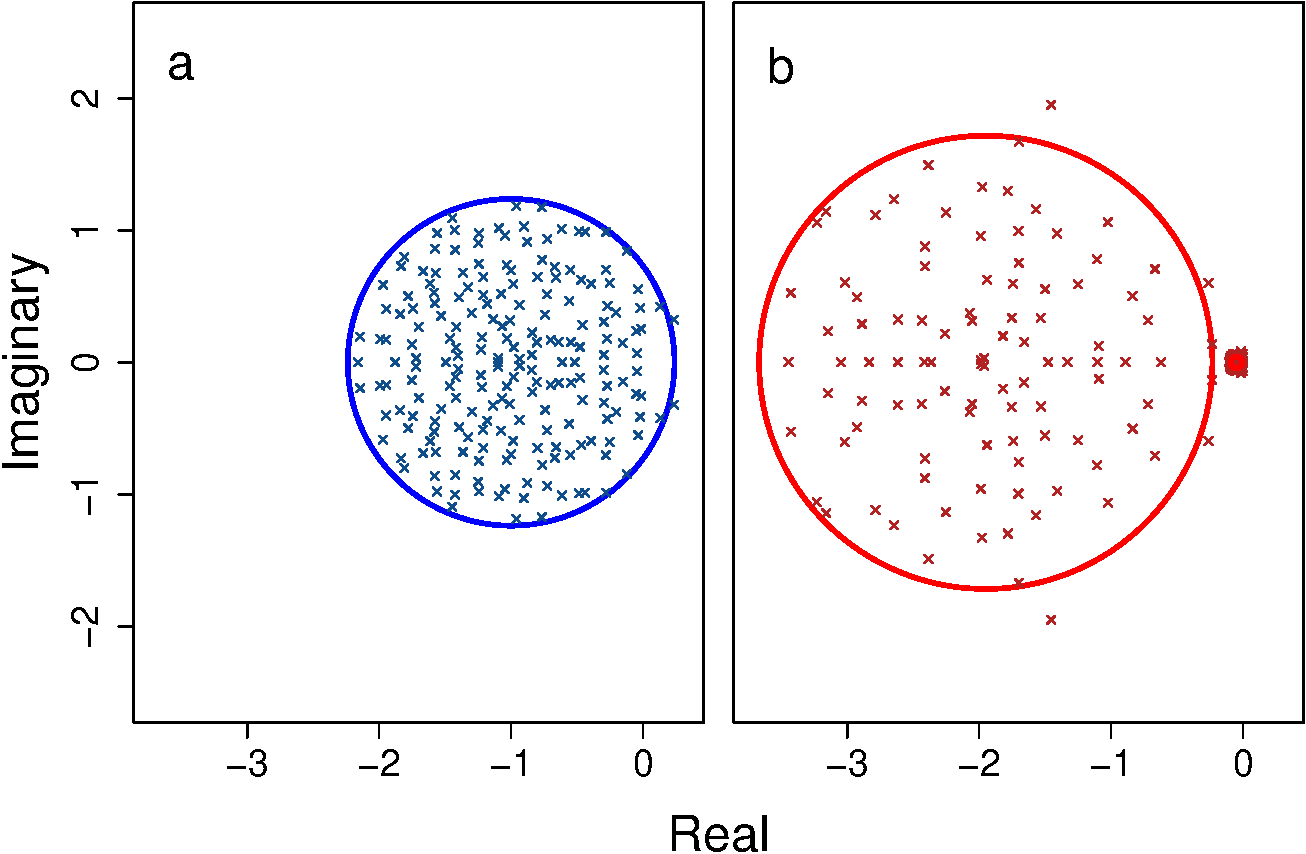
\includegraphics{ms_files/figure-latex/unnamed-chunk-10-1.pdf}

\clearpage

\textbf{Figure 2: Distributions of eigenvalues before (a) and after (b)
introducing variation in component response rate
(\(\boldsymbol{\gamma}\)) in complex systems.} Each panel show the same
system where \(S = 1000\), \(C = 0.05\), and \(\sigma = 0.4\).
\textbf{a.} Eigenvalues plotted in the absence of \(Var(\gamma)\) where
\(E[\gamma] = 1\), versus \textbf{b.} eigenvalues plotted given
\(\gamma \sim \mathcal{U}(0, 2)\), which increases the variance of
interaction strengths (\(\sigma^{2}\)) but also creates a cluster of
eigenvalues toward the distribution's centre (-1, 0). Blue elipses in
both panels show the circle centred on the distribution in panel a.
Proportions of \(\Re(\lambda) < 0\) are 0.723 and 0.737 for a and b,
respectively.

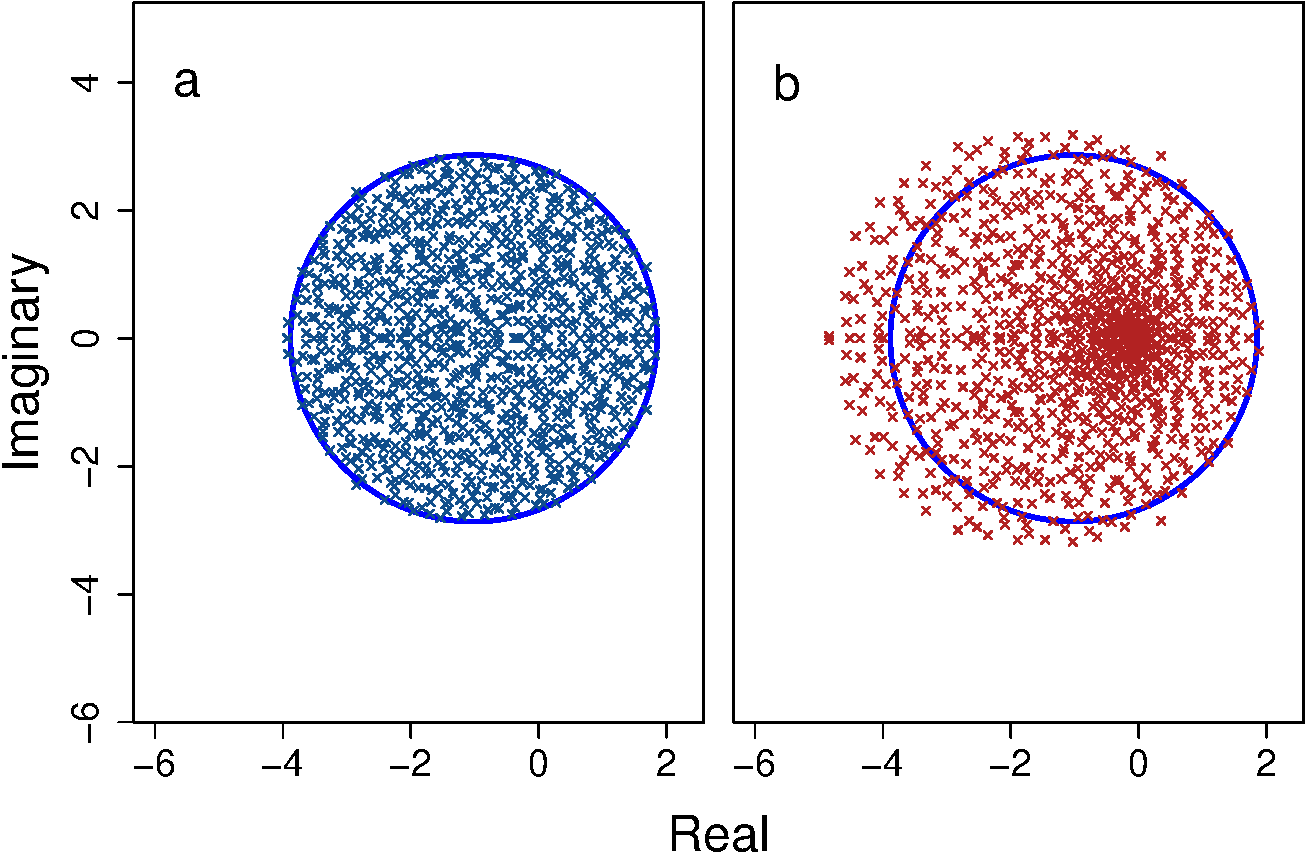
\includegraphics{ms_files/figure-latex/unnamed-chunk-13-1.pdf}

\clearpage

\textbf{Figure 3: Stability of large complex systems with and without
variation in component response rate (\(\boldsymbol{\gamma}\)).} The
\(\ln\) number of systems that are stable across different system sizes
(\(S\), max \(S=50\)) given \(C = 1\), and the proportion of systems in
which variation in \(\gamma\) is critical for system stability. For each
\(S\), 1 million complex systems are randomly generated. Stability of
each complex system is tested given variation in \(\gamma\) by randomly
sampling \(\gamma \sim \mathcal{U}(0, 2)\). Stability given
\(Var(\gamma)\) is then compared to stability in an otherwise identical
system in which \(\gamma = E[\mathcal{U}(0, 2)]\) for all components.
Blue and red bars show the number of stable systems in the absence and
presence of \(Var(\gamma)\), respectively. The black line shows the
proportion of systems that are stable when \(Var(\gamma) > 0\), but
would be unstable if \(Var(\gamma) = 0\).

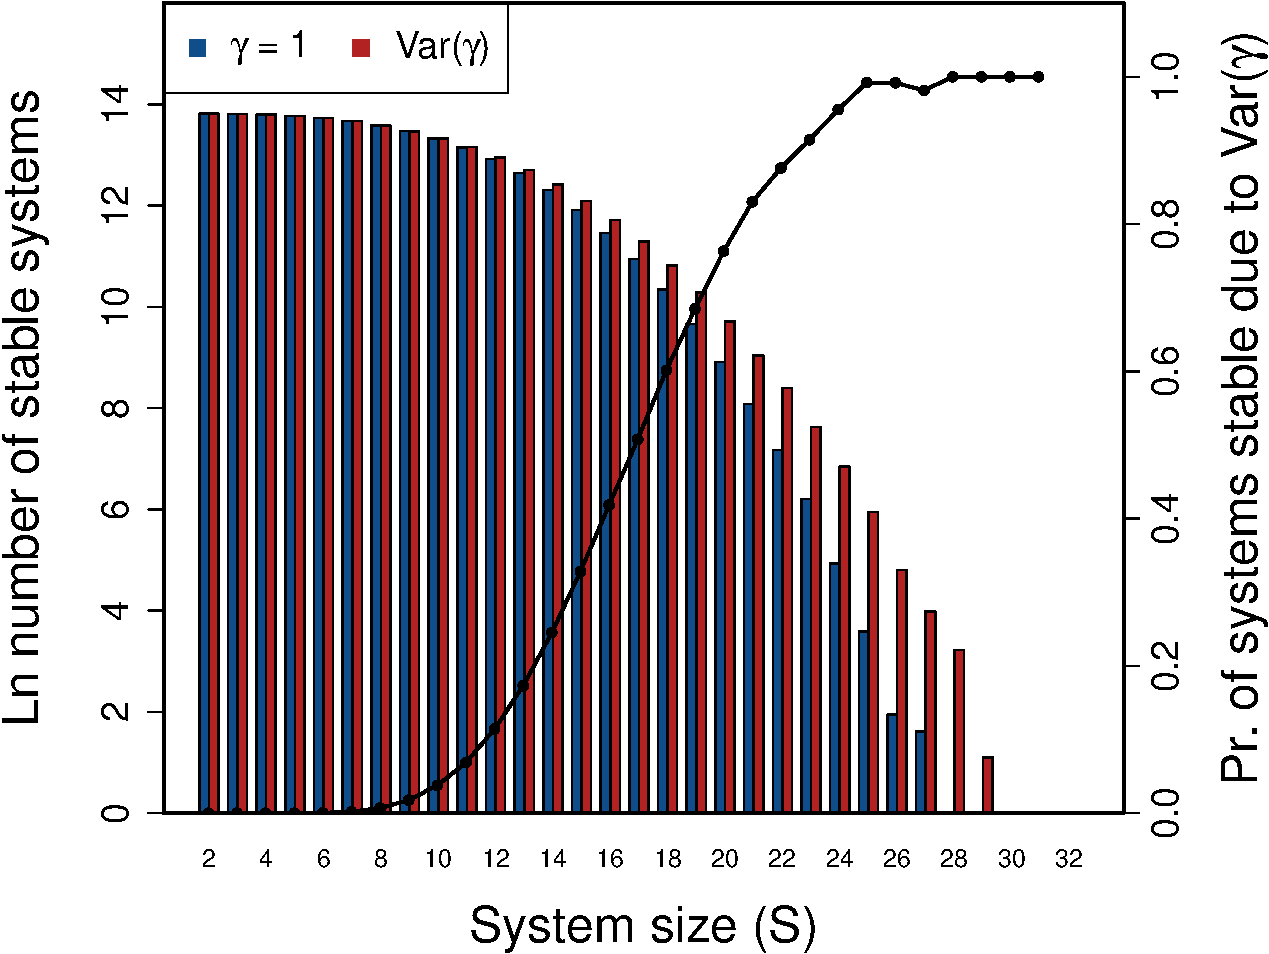
\includegraphics{ms_files/figure-latex/unnamed-chunk-15-1.pdf}

\clearpage

\textbf{Figure 4: Stability of large complex systems given
\(\boldsymbol{\gamma = 1}\) versus targeted
\(\boldsymbol{Var(\gamma)}\).} The \(\ln\) number of systems that are
stable across different system sizes (\(S\), max \(S=40\)) for
\(C = 1\), and the proportion of systems wherein a targeted search of
\(\gamma\) values successfully resulted in system stability. For each
\(S\), 100000 complex systems are randomly generated. Stability of each
complex system is tested given variation in \(\gamma\) using a genetic
algorithm to maximise the effect of \(\gamma\) values on increasing
stability, as compared to stability in an otherwise identical system in
which \(\gamma\) is the same for all components. Blue bars show the
number of stable systems in the absence of component response rate
variation, while red bars show the number of stable systems that can be
generated if component response rate is varied to maximise system
stability. The black line shows the proportion of systems that are
stable when component response rate is targeted to increase stability,
but would not be stable if \(Var(\gamma) = 0\).

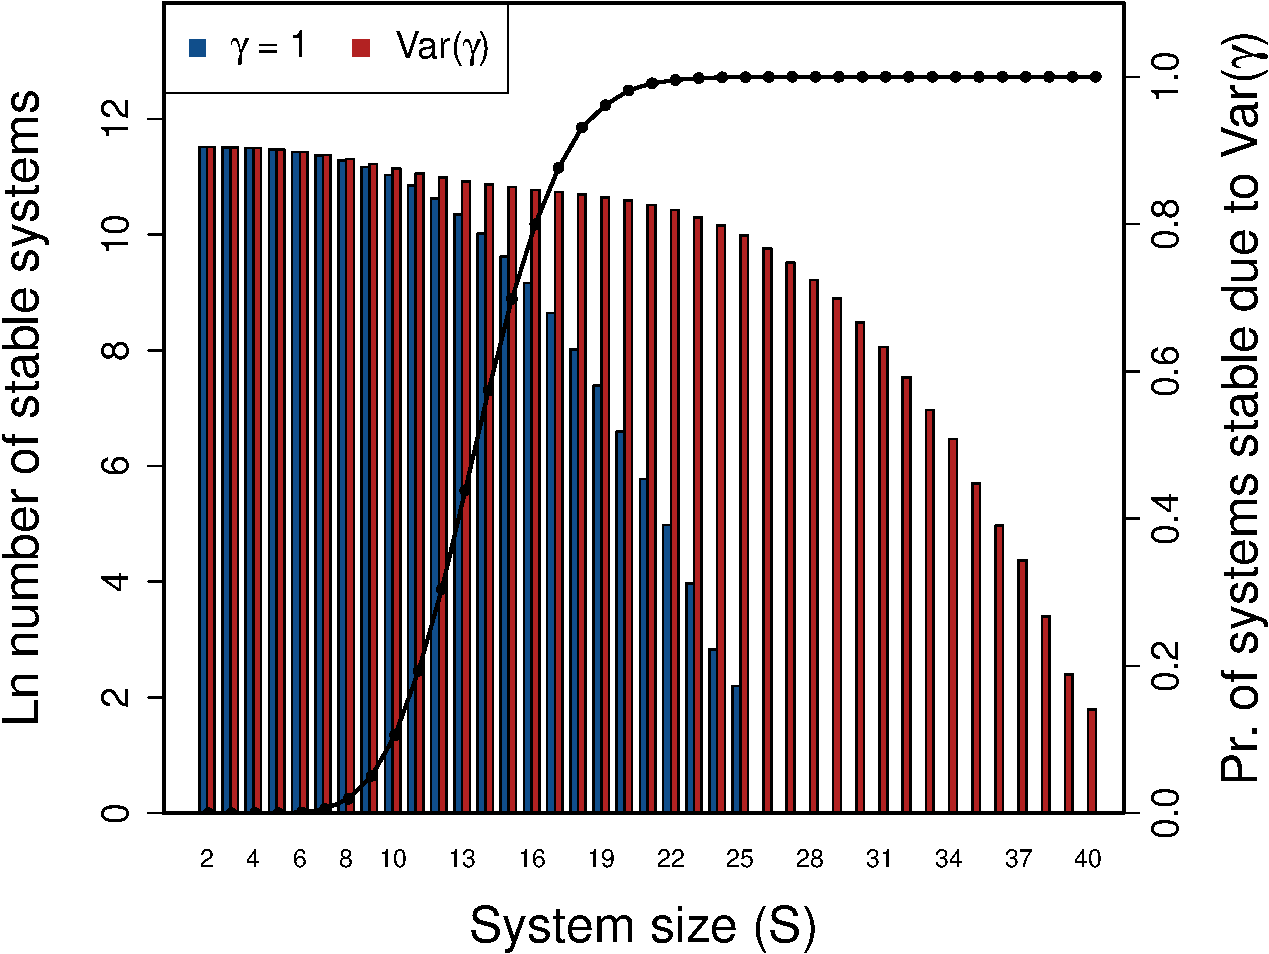
\includegraphics{ms_files/figure-latex/unnamed-chunk-16-1.pdf}


\end{document}
